\section{OracleGate Case Studies}
\label{app:og-vignettes}

To make concrete what the \textsc{OracleGate} upper-bound result looks like at the
episode level, we enumerate a few representative paired tuples from the
$N{=}300$ low-light severity~$4$~seed~$0$ comparison. Each row is the \emph{same}
episode evaluated under three arms in lock-step; ``$\checkmark$'' marks success.

\begin{table}[h]
\centering
\small
\setlength{\tabcolsep}{3.5pt}
\begin{tabular}{llcccccc}
\toprule
ID & Type & Goal & B0 & RES & OG & DTG (OG / B0) \\
\midrule
R1 & \emph{rescued} & sofa & $\times$ & $\times$ & \checkmark & $0.06$ / $2.36$ \\
R2 & \emph{rescued} & bed & $\times$ & $\times$ & \checkmark & $0.03$ / $7.76$ \\
R3 & \emph{rescued} & chair & $\times$ & $\times$ & \checkmark & $0.04$ / $3.75$ \\
R4 & \emph{rescued} & bed & $\times$ & $\times$ & \checkmark & $0.15$ / $7.80$ \\
\midrule
K1 & \emph{broken} & chair & $\times$ & \checkmark & $\times$ & $7.57$ / $0.06$ \\
K2 & \emph{broken} & television set & $\times$ & \checkmark & $\times$ & $2.05$ / $6.81$ \\
K3 & \emph{broken} & potted plant & $\times$ & \checkmark & $\times$ & $2.49$ / $0.14$ \\
\midrule
T1 & \emph{tied} & toilet & $\times$ & $\times$ & $\times$ & $1.78$ / $0.02$ \\
T2 & \emph{tied} & chair & $\times$ & $\times$ & $\times$ & $3.23$ / $0.15$ \\
\bottomrule
\end{tabular}
\caption{Per-episode case studies on the $N{=}300$ low-light cell.
\textbf{Rescued}~(R1--R4): both deployable arms (B0, RES) fail and the
non-deployable per-frame appearance oracle (\textsc{OracleGate}, OG)
succeeds; the upper-bound oracle reaches the goal at a meaningfully
closer distance.
\textbf{Broken}~(K1--K3): RES already succeeded, but OG, by greedy
per-frame view selection, lands on the wrong commitment and the
trajectory diverges; over the full $N{=}300$ cell OG breaks
$b_{10}{=}36$ RES-successes while rescuing
$b_{01}{=}41$ RES-failures, leaving the net paired
$\Delta\text{SR}_{\text{OG--RES}}{=}+0.017$.
\textbf{Tied}~(T1--T2): all three arms fail with similar final DTG; the
degradation has destroyed information that no oracle over the same RGB
channel can recover. Bucket sizes: rescued $n_{R}{=}21$,
broken $n_{K}{=}36$,
all-failed (tied) $n_{T}{=}128$, out of $N{=}300$.}
\label{tab:og-vignettes}
\end{table}

The vignette table makes the headline OracleGate observation visible at
the case level: even a per-frame appearance oracle, exempt from runtime
reliability estimation, has to \emph{break} nearly as many episodes as it
\emph{rescues} ($b_{01}{=}41$ vs $b_{10}{=}36$ when paired against RES),
leaving the paired $\Delta$SR over RES at only $+0.017$.
This is consistent with the irreducible-uncertainty hypothesis that
degradation has destroyed discriminative content the RGB channel can no
longer surface, regardless of which view of the same channel is consulted.

\begin{figure*}[t]
\centering
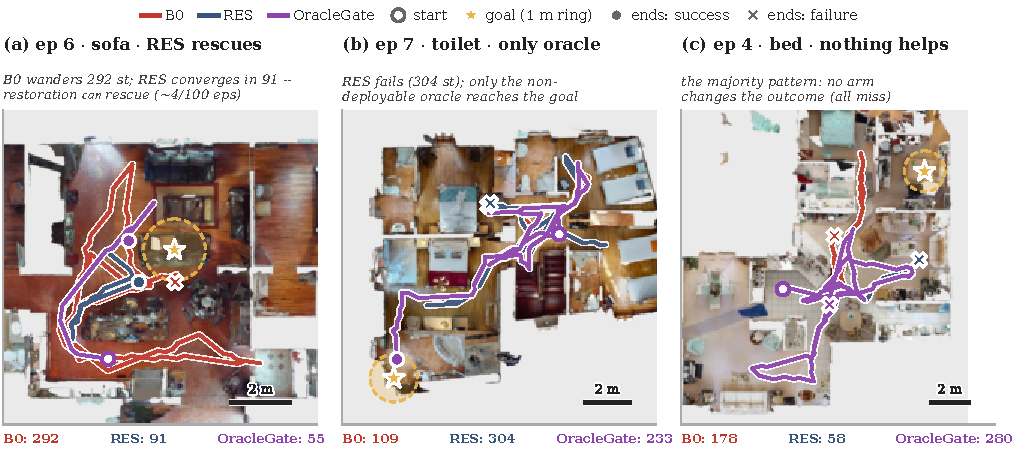
\includegraphics[width=0.98\textwidth]{figures/fig_topdown_traj.pdf}
\caption{\textbf{Multi-arm top-down trajectories on three matched episodes}
(a $12$-episode sub-sample of the low-light severity~$4$~seed~$0$ paired
list). Each panel is a bird's-eye orthographic render of the actual HM3D
scene (ceiling clipped) with the logged per-step world positions of the
B0, RES, and \textsc{OracleGate} agents overlaid; the star and 1\,m
ring mark the ObjectNav success radius, and the terminal marker is a dot
(success) or cross (failure). \textbf{(a)}~ep~6, a scenario where
restoration \emph{can} rescue: B0 wanders for 292 steps, RES converges in
91 with the same commit rule. \textbf{(b)}~ep~7, a scenario the deployable
restoration cannot fix: RES still fails after 304 steps and only the
non-deployable per-frame appearance oracle reaches the goal.
\textbf{(c)}~ep~4, the majority pattern of the $N{=}300$ sweep: all three
arms diverge into different corners of the same scene and none of them
lands inside the success ring---the low-light corruption has destroyed
discriminative content that no RGB-side lever can recover. The three
panels concretise the bucket sizes reported in
Table~\ref{tab:og-vignettes}: 21 out of 300 rescued, 36 out of 300 broken,
and 128 out of 300 tied all-failed.}
\label{fig:topdown-traj}
\end{figure*}

